

\section{Prototipação da Interface do Usuário}

\subsection{Objetivo da Prototipação}

A prototipação foi utilizada como estratégia para validar os fluxos de uso, testar a usabilidade da interface e antecipar problemas relacionados à disposição dos elementos, acessibilidade e validações essenciais na interação do usuário com o sistema \textit{SAMGestor}. Esta etapa foi fundamental para assegurar que a camada de apresentação estivesse alinhada com as regras de negócio e necessidades operacionais identificadas durante o levantamento de requisitos.

O protótipo permitiu simular, de forma visual e interativa, os principais módulos do sistema, como inscrições, contemplações, pagamentos, formações de famílias, organização de barracas, equipes de serviço e envio de mensagens. Além disso, garantiu que as restrições de acesso por perfil de usuário fossem corretamente representadas e validadas.

\subsection{Fluxo Geral de Interação}

Os itens abaixo representaram o fluxo principal da aplicação, conforme será observado nos protótipos:

\begin{enumerate}
    \item Usuário não logado acessa o formulário público de inscrição.
    \item Gestor cria o retiro e configura parâmetros básicos.
    \item Gestor importa inscrições ou cadastra individualmente.
    \item Gestor realiza a contemplação dos inscritos.
    \item Envia mensagens solicitando confirmação.
    \item Usuário confirma ou desiste; sistema marca como “Pagamento Pendente”.
    \item Realização do pagamento automático ou manual com upload do comprovante.
    \item Composição de famílias (manual ou sorteio).
    \item Organização das barracas e equipes de serviço.
    \item Visualização de relatórios e indicadores no dashboard.
\end{enumerate}

\subsection{Considerações Finais}

Todas as telas que envolvem operações do tipo CRUD devem seguir rigorosamente as validações de campos obrigatórios e manter coerência entre entidades relacionadas. A aplicação foi pensada para ser responsiva, garantindo acesso eficiente via dispositivos móveis, especialmente para o formulário de inscrição.

As regras descritas nesta seção orientaram diretamente a implementação do protótipo de interface, garantindo usabilidade, clareza e segurança em todos os fluxos de interação no contexto da gestão de retiros espirituais.

\subsection{Ferramentas Utilizadas}

Para a criação dos protótipos da interface do sistema, foi utilizada a ferramenta \textbf{Figma}, que possibilitou a elaboração de protótipos navegáveis de alta fidelidade. Essa abordagem permitiu simular, de forma precisa, as principais funcionalidades da aplicação, proporcionando uma visualização realista da experiência do usuário antes da implementação do \textit{front-end} definitivo.

Segundo a documentação oficial do Figma, a ferramenta destaca-se por permitir a colaboração em tempo real, integração com fluxos de desenvolvimento ágil e facilidade na criação de protótipos interativos acessíveis via navegador, sem necessidade de instalação local. Tais características a tornam especialmente adequada para projetos educacionais e profissionais que exigem validação constante com stakeholders \cite{figma_docs}.

\subsection{Tipos de Protótipo}

Todos os protótipos desenvolvidos para este trabalho foram de \textbf{alta fidelidade}, com layouts e elementos visuais que simulam de forma precisa a interface final do sistema. Além do aspecto visual refinado, alguns desses protótipos foram dotados de interatividade, permitindo ao usuário navegar entre as telas e experimentar fluxos reais de uso, como se estivesse utilizando o sistema já implementado.

A escolha por protótipos de alta fidelidade se justifica pela necessidade de validar aspectos detalhados da experiência do usuário (\textit{UX}), como disposição de componentes, legibilidade, fluxo de navegação, acessibilidade e consistência visual. Esses protótipos também serviram como referência direta para a implementação do \textit{front-end}, reduzindo ambiguidades e facilitando a comunicação entre os envolvidos no projeto.

\subsection{Apresentação dos Protótipos}

A seguir, são apresentadas algumas das telas desenvolvidas durante a fase de prototipação, com o objetivo de ilustrar a estrutura visual e os principais fluxos de navegação do sistema. Os protótipos foram criados com foco na simplicidade, clareza e acessibilidade, alinhando-se às regras de negócio e perfis de usuário definidos.

\begin{figure}[H]
\centering
\includegraphics[width=0.8\textwidth]{images/prototipacao/gestao_de_usuarios/Gestão de Usuarios.png}
\caption{Tela inicial da gestão de usuários com funcionalidades de visualização, edição, criação e remoção.}
\end{figure}

\begin{figure}[H]
\centering
\includegraphics[width=0.8\textwidth]{images/prototipacao/gestao_de_usuarios/Editar Usuário.png}
\caption{Formulário de criação ou edição do usuário}
\end{figure}

\begin{figure}[H]
\centering
\includegraphics[width=0.8\textwidth]{images/prototipacao/gestao_de_usuarios/Permissões de Usuarios.png}
\caption{Tela onde serão apresentadas as permissões do usuário, onde o Administrador poderá estar ativando ou desativando de forma personalizada os acessos que o usuário terá no sistema.}
\end{figure}

\begin{figure}[H]
\centering
\includegraphics[width=0.8\textwidth]{images/prototipacao/gestao_de_usuarios/Permissões obrigatórias do cargo.png}
\caption{Na tela de permissões, as permissões referentes ao cargo não poderão ser modificadas.}
\end{figure}

\begin{figure}[H]
\centering
\includegraphics[width=0.8\textwidth]{images/prototipacao/gestao_de_usuarios/Credenciais do Usuário.png}
\caption{Tela destinada à redefinição de credenciais de usuários por um administrador do sistema. Esta funcionalidade é utilizada em casos nos quais o usuário perdeu o acesso e não possui e-mail confirmado para recuperação. Por questões de segurança e privacidade, o administrador não visualiza as credenciais atuais do usuário — apenas define valores provisórios. Ao realizar o primeiro acesso com as novas credenciais, o próprio usuário será solicitado a redefini-las. O acesso a esta funcionalidade requer autenticação adicional do administrador mediante digitação da sua senha.}
\end{figure}

\begin{figure}[H]
\centering
\includegraphics[width=0.8\textwidth]{images/prototipacao/gestao_retiros_geral/Gestão de Retiros Geral.png}
\caption{Tela inicial do módulo de gestão de retiros. Apresenta funcionalidades para visualização, edição, criação e exclusão de registros de retiros, permitindo ao usuário administrador gerenciar eficientemente os eventos cadastrados no sistema.}
\end{figure}

\begin{figure}[H]
\centering
\includegraphics[width=0.8\textwidth]{images/prototipacao/gestao_retiros_geral/Ver Mais Retiro.png}
\caption{Ao clicar no botão "Ver mais", uma modal com informações do retiro é aberta.}
\end{figure}

\begin{figure}[H]
\centering
\includegraphics[width=0.8\textwidth]{images/prototipacao/gestao_retiros_geral/Geral.png}
\caption{Formulário de criação ou edição do retiro.}
\end{figure}

\begin{figure}[H]
\centering
\includegraphics[width=0.8\textwidth]{images/prototipacao/gestao_retiros_geral/Formulario.png}
\caption{Ferramenta para criação de formulários, onde o gestor irá decidir o título, descrição, ordem e nome dos campos.}
\end{figure}

\begin{figure}[H]
\centering
\includegraphics[width=0.8\textwidth]{images/prototipacao/gestao_retiros_geral/FormularioEquipeDeServico.png}
\caption{Aba de criação do formulário para a equipe de serviço.}
\end{figure}

\begin{figure}[H]
\centering
\includegraphics[width=0.8\textwidth]{images/prototipacao/gestao_retiros_geral/Ajuda.png}
\caption{Modal de ajuda com informações de como utilizar a ferramenta construtura de formulários.}
\end{figure}

\begin{figure}[H]
\centering
\includegraphics[width=0.8\textwidth]{images/prototipacao/gestao_retiros_geral/NaoContemplados.png}
\caption{Tabela de participantes não contemplados. Permite ao gestor visualizar os inscritos ainda não selecionados para o retiro. Através do menu de contexto (acesso via botão direito do mouse), é possível contemplar o participante ou acessar detalhes adicionais por meio da opção "Ver mais informações".}
\end{figure}

\begin{figure}[H]
\centering
\includegraphics[width=0.8\textwidth]{images/prototipacao/gestao_retiros_geral/Contemplados-1.png}
\caption{Tabela de participantes contemplados. Exibe a lista de participantes já selecionados para o retiro. Por meio do menu de contexto (acesso via clique com o botão direito do mouse), o gestor pode abrir o modal de envio de mensagem ou visualizar informações detalhadas do participante.}
\end{figure}

\begin{figure}[H]
\centering
\includegraphics[width=0.8\textwidth]{images/prototipacao/gestao_retiros_geral/ContemplaçãoModal.png}
\caption{Modal de envio de mensagens personalizadas. Permite ao gestor compor e enviar mensagens personalizadas para participantes contemplados, com suporte ao envio em lote para múltiplos destinatários simultaneamente.}
\end{figure}

\begin{figure}[H]
\centering
\includegraphics[width=0.8\textwidth]{images/prototipacao/gestao_retiros_geral/Pendentes.png}
\caption{Tabela com participantes contemplados com filtro de participação não confirmada.}
\end{figure}

\begin{figure}[H]
\centering
\includegraphics[width=0.8\textwidth]{images/prototipacao/form_publico/listVierPage.png}
\caption{Página inicial com os retiros.}
\end{figure}

\begin{figure}[H]
\centering
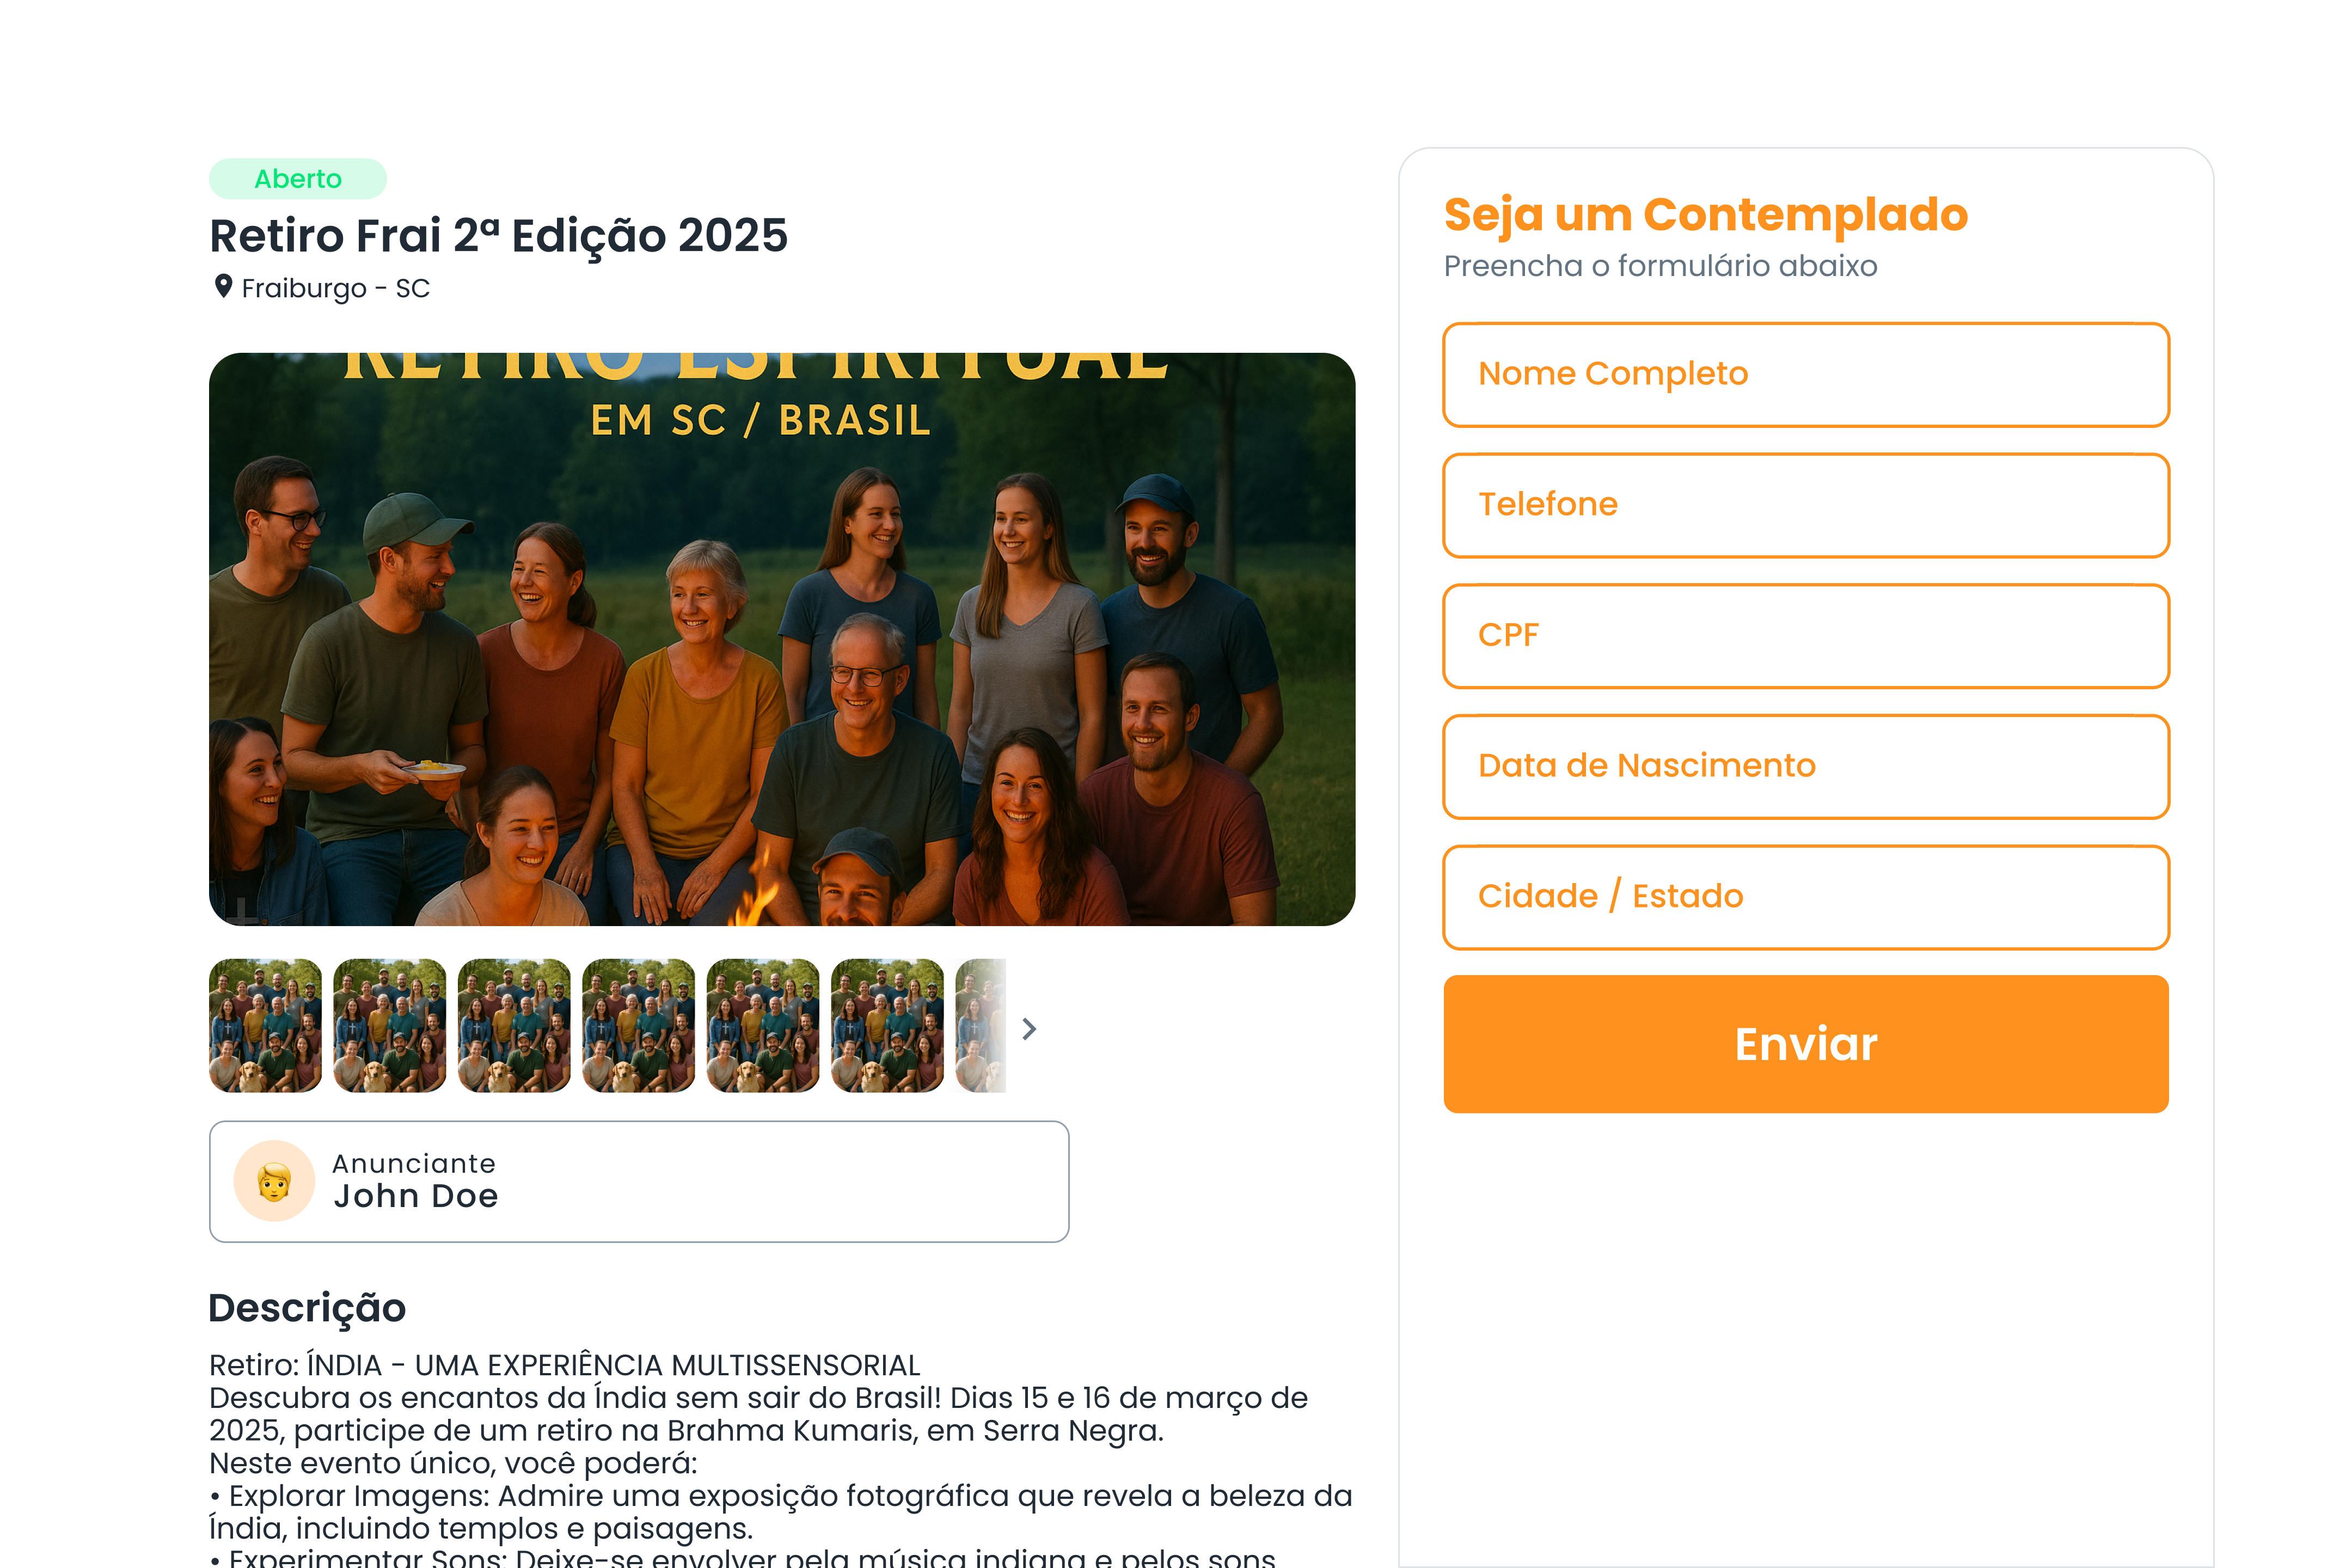
\includegraphics[width=0.8\textwidth]{images/prototipacao/form_publico/Detail Page - Retiro.png}
\caption{Página com os detalhes do retiro e o formulário.}
\end{figure}

\begin{figure}[H]
\centering
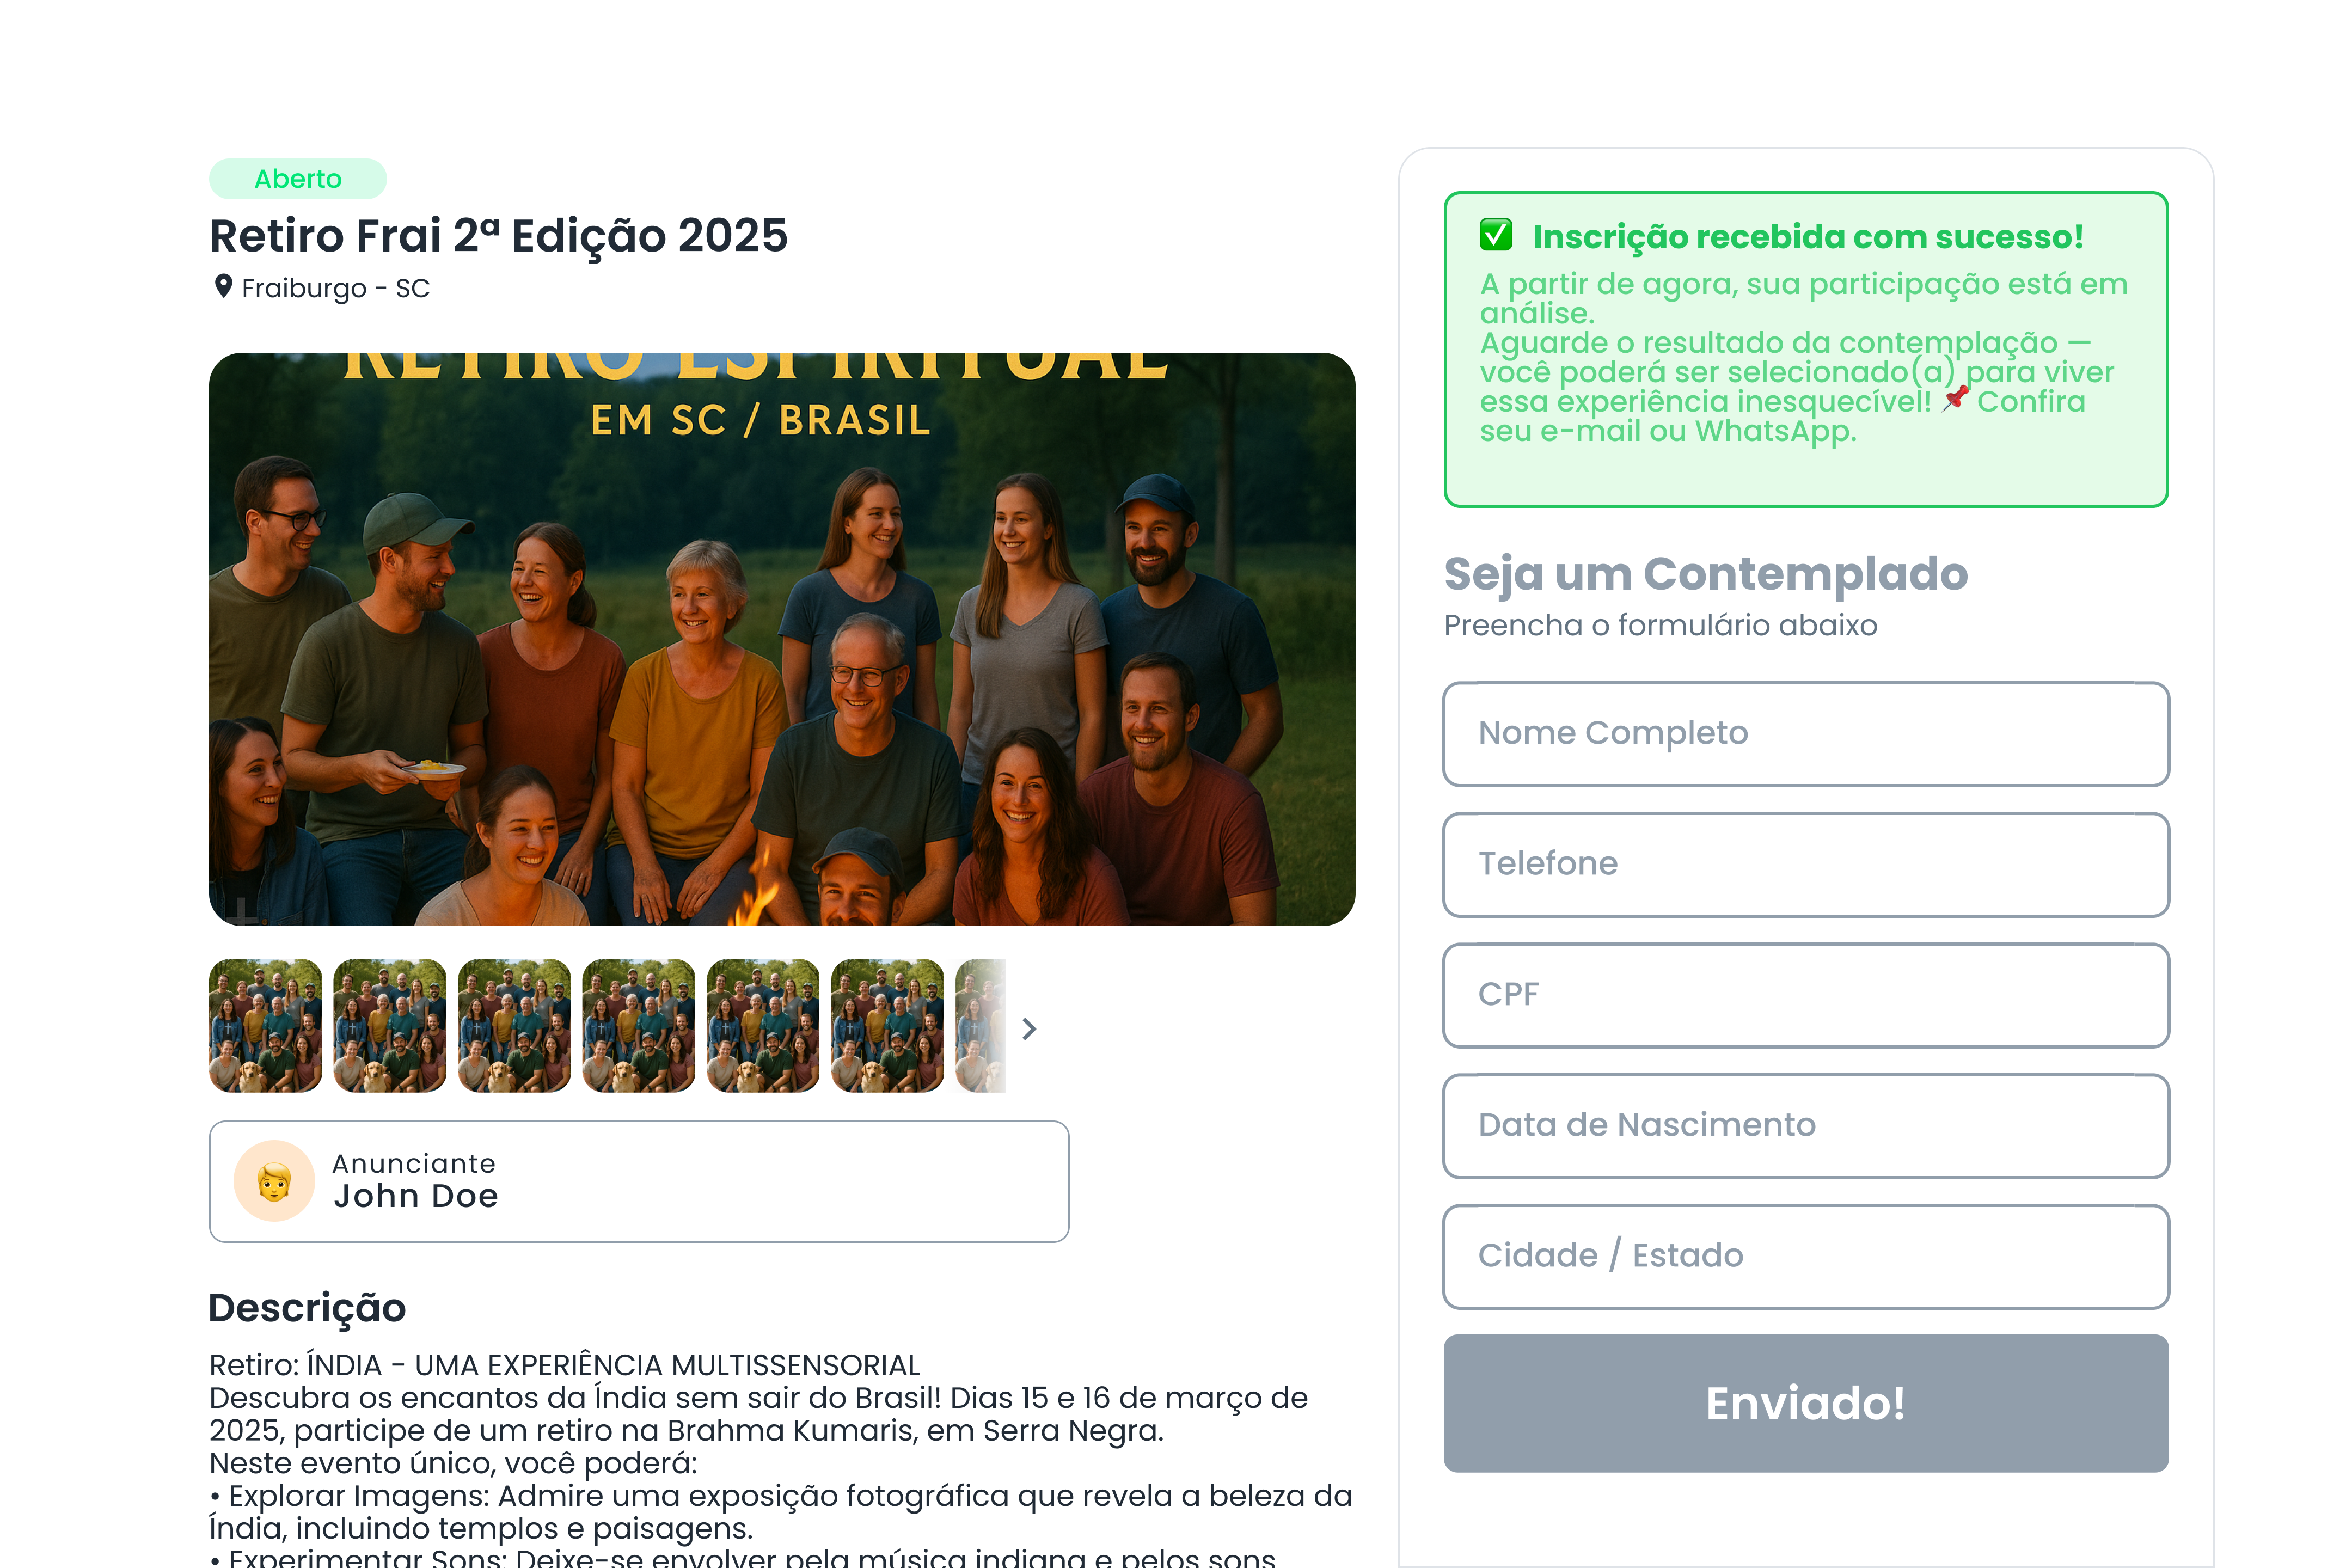
\includegraphics[width=0.8\textwidth]{images/prototipacao/form_publico/Detail Page - Retiro (Success).png}
\caption{Mensagem de sucesso exibida após o envio do formulário. Informa ao usuário que o preenchimento foi concluído com êxito e os dados foram processados corretamente.}
\end{figure}

\begin{figure}[H]
\centering
\includegraphics[width=0.8\textwidth]{images/prototipacao/participant_login/register.png}
\caption{Página de registro para participantes contemplados. Permite que o participante selecionado para o retiro crie sua conta de acesso ao sistema, inserindo suas informações pessoais e definindo suas credenciais de autenticação.}
\end{figure}

\begin{figure}[H]
\centering
\includegraphics[width=0.8\textwidth]{images/prototipacao/participant_login/login.png}
\caption{Pagina de login geral dos usuários.}
\end{figure}

\begin{figure}[H]
    \centering
    \includegraphics[width=0.8\textwidth]{images/prototipacao/participant_login/forgotpassword.png}
    \caption{Pagina de recuperacão das credenciais.}
    \end{figure}

\begin{figure}[H]
\centering
\includegraphics[width=0.8\textwidth]{images/prototipacao/participant_login/HomePage.png}
\caption{Paginá inicial do participante que irá pagar o retiro de forma automática.}
\end{figure}

\begin{figure}[H]
\centering
\includegraphics[width=0.8\textwidth]{images/prototipacao/participant_login/Payment Page - Retiro.png}
\caption{Escolha do pagamento no formato de crédito.}
\end{figure}

\begin{figure}[H]
\centering
\includegraphics[width=0.8\textwidth]{images/prototipacao/participant_login/Payment Page - Retiro-1.png}
\caption{Escolha do pagamento no formato de PIX.}
\end{figure}


\begin{figure}[H]
\centering
\includegraphics[width=0.8\textwidth]{images/prototipacao/familia/Familias-3.png}
\caption{Tela inicial das famílias.}
\end{figure}

\begin{figure}[H]
\centering
\includegraphics[width=0.8\textwidth]{images/prototipacao/familia/Familias-2.png}
\caption{Avisos de erros na composição de uma família.}
\end{figure}

\begin{figure}[H]
\centering
\includegraphics[width=0.8\textwidth]{images/prototipacao/familia/Familias-1.png}
\caption{Adição de um participante na família.}
\end{figure}

\begin{figure}[H]
\centering
\includegraphics[width=0.8\textwidth]{images/prototipacao/familia/Familias.png}
\caption{Adição de múltiplos participantes na família.}
\end{figure}

\begin{figure}[H]
\centering
\includegraphics[width=0.8\textwidth]{images/prototipacao/barracaEequipeDeServico/Equipes de serviço.png}
\caption{Tela inicial das equipes de serviço.}
\end{figure}

\begin{figure}[H]
\centering
\includegraphics[width=0.8\textwidth]{images/prototipacao/barracaEequipeDeServico/Gestão de Barracas.png}
\caption{Tela inicial das barracas.}
\end{figure}

\begin{figure}[H]
\centering
\includegraphics[width=0.8\textwidth]{images/prototipacao/relatorios/Relatórios-1.png}
\caption{Tela inicial dos relatórios.}
\end{figure}

\begin{figure}[H]
\centering
\includegraphics[width=0.8\textwidth]{images/prototipacao/relatorios/Relatórios.png}
\caption{Formulário para edição ou criação dos relatórios.}
\end{figure}

\begin{figure}[H]
\centering
\includegraphics[width=0.8\textwidth]{images/prototipacao/relatorios/Gestão de Usuarios.png}
\caption{Resultado dos filtros.}
\end{figure}

\begin{figure}[H]
\centering
\includegraphics[width=0.8\textwidth]{images/prototipacao/relatorios/Gestão de Usuarios-1.png}
\caption{Configuração dos filtros.}
\end{figure}

\begin{figure}[H]
\centering
\includegraphics[width=0.8\textwidth]{images/prototipacao/notificacoes/Notificações.png}
\caption{Painel lateral de notificações do sistema. Exibe alertas e mensagens relevantes ao usuário, incluindo atualizações sobre inscrições, contemplações, pagamentos e outras ações realizadas no sistema.}
\end{figure}

\begin{figure}[H]
\centering
\includegraphics[width=0.8\textwidth]{images/prototipacao/notificacoes/Notificações-1.png}
\caption{Popover  com botões para acessar as configurações das notificações.}
\end{figure}

\begin{figure}[H]
\centering
\includegraphics[width=0.8\textwidth]{images/prototipacao/notificacoes/notificacoesmodal.png}
\caption{Modal com as configurações das notificaões.}
\end{figure}


Esses protótipos possibilitaram validar a experiência do usuário em diferentes perfis de acesso (Administrador, Gestor e Consultor), além de antecipar ajustes visuais e comportamentais antes da implementação do sistema. Os fluxos de navegação detalhados estão documentados por meio de diagramas de sequência no capítulo correspondente.
O protótipo completo da interface, com todos os fluxos interativos detalhados, está disponível no \textbf{Anexo A}.f